\section{Packet Streaming} \label{sec:terminologies}

\hbadd{In order to systematically study the resolution-versus-precision
tradeoffs, it is important to compare different data reduction techniques.}
One popular method is to restrict the techniques to the same data size and
compare data quality. It is, however, difficult to enforce that a
multiresolution scheme uses the same amount of data as does quantization scheme,
because \hbadd{the amount of data change in one step of multiresolution
simplification may be different from removing one bit in the quantization of
every data sample.} \hbdel{going down one step in resolution decreases the data
size by a different amount than when removing one more bit from each data
sample.} To avoid such mismatch of data increment/decrement units, we model
each reduction scheme as a stream of equally-sized \emph{packets}.  We define a
packet as the smallest unit of data increment/decrement in our framework, with
each packet consisting of a relatively small number of bits from a data set. To
study the resolution-versus-precision tradeoffs, we associate a packet with a
resolution level and a precision level (i.e., bit plane), so that each packet
can improve either data's resolution or its precision. In this framework,
different data reduction schemes become different orderings of packets from a
data set, or different packet \emph{streams}.  For example, a quantization
scheme would stream packets by precision, whereas a multiresolution scheme would
stream packets by resolution. By forcing the different schemes to use the same
number of packets, we can compare data quality across the schemes fairly.

In \Cref{sec:data-streaming-framework}, we discuss the mechanism of converting
original data into a set of packets. \Cref{sec:static-dynamic-streams}
describes packet streams that correspond to common data reduction schemes.
\Cref{sec:data_dep_streams} presents a greedy algorithm to approximate the
optimal packet stream for the data and the analysis task at hand. Finally,
\Cref{sec:stream-signature} introduces a novel concept called \emph{stream
signature} that can be used to study and compare the characteristics of
different packet streams.

\subsection{Decomposition of Data into Packets} \label{sec:data-streaming-framework}

Each new packet adds to the data's resolution and/or precision. To introduce
the concept of resolution, we use the popular CDF5/3 discrete wavelet transform
\todo{[CITE]}.  Although there exist other transforms that separate a signal
into discrete bands of frequencies/scales/resolutions, such as the discrete
Fourier transform, we choose wavelet transform because wavelet coefficients are
spatially localized. This localization enables spatial adaptivity, allowing
finer resolution in regions that contain \hbadd{sharp} \hbdel{important}
features, at the expense of coarser resolution elsewhere. The hierarchical-Z
indexing scheme \todo{[CITE]} also produces a multiresolution representation,
but unlike wavelets, it offers no interpolation mechanism for low-resolution
grids. We choose the CDF5/3 wavelet for its balance between simplicity and
effectiveness at decorrelating the input signal. It is also one of the two
transforms of choice in the JPEG2000 standard~\cite{jpeg2001}.

The \hbdel{typical} multidimensional wavelet transform can be performed in
multiple passes, which eventually results in the original domain being
partitioned into several \emph{subbands}, each of which can be thought of as a
resolution level. One transform pass creates four subbands in 2D and eight in
3D, of which the first is a smoothed, downsampled version of the original data.
The next seven subbands (in 3D) add fine details in each subset of the
dimensions. A subsequent transform pass \hbdel{typically} recurses on the first
subband created by the previous pass, leaving the other seven subbands intact.
We \hbdel{frequently} use $l$ $(0 \leq l < L)$ to index the subbands, with $l =
0$ referring to the coarsest subband, and $L$ \hbadd{denotes the number of
subbands.} \hbdel{to denote the highest indexed subband.} In this paper, we use
\hbadd{$L=22$} \hbdel{$L=21$} (in 3D), corresponding to three transform passes.
\hb{changed the defn of $L$ to make it consistent with $B$
in the next paragraph}

For \hbadd{creating packets corresponding to different} precision, we quantize
floating-point wavelet coefficients to $B$-bit signed integers. For most of the
experiments in this paper, $B=16$. This quantization eliminates the exponent
bits, such that every bit (except the sign bit) can be associated with a bit
plane $b$ ($0\leq b < B$), contributing $2^b$ in absolute value to its
coefficient's value. To avoid special treatment of the sign bit, we
convert quantized coefficients from two's complement form to a negabinary form,
in which integers are represented in base $-2$, i.e.,
$\sum_{i=0}^{B}{c_i(-2)^i}$ with $c_i\in \{0,1\}$. This transformation
increases the number of bit planes by one, to compensate for the absence of the
sign bit.  \hbadd{In the negabinary form, the higher indexed bit planes are
less significant.} \hbdel{We use $b$, which starts from 0, to index the bit
planes, with the convention that higher indexed bit planes are less
significant.} \hb{$b$ as the index is already defined, so no need to repeat.
however, if i understand correctly, the meaning of $b$ changes after converting
to negabinary, so that needs pointing out}

As mentioned earlier, the smallest unit of data in our framework is called a
\emph{packet}.  More precisely, a packet consists of bits on the same bit
plane, from a \emph{block} of negabinary wavelet coefficients. A block is a
$g\times g\times g$ grid of adjacent coefficients on the same subband. We let
$g$ be a constant, so that finer resolution subbands contain more packets. This fixed size
enables the natural tradeoff between wider (but coarser) coverage and finer
(but more local) details, for the same number of packets\pavol{unclear what you mean here}. In this paper, a
packet always contains $4096$ bits (i.e., $g=16$), following the common
practice of reading bits in batches for performance reason. This choice of $g$
also accelarates our experiments significantly, without affecting the results
in a meaningful way. \hb{this paragraph has some info missing. here, a packet
combinse both resolution and precision, right. i can rephrase after some
clarification.}

A data reduction scheme can be modeled as an ``inverse'' stream of packets,
where the original data contains all packets, and any reduction step removes
certain packets based on some criteria (details in
\Cref{sec:static-dynamic-streams}).  \hbadd{These data streams are provided
using a client-server model.} \hbdel{In our data streaming model, there is a
``server'' that serves data and a ``client'' that receives data from the
server.} At any point, the client is assumed to have received a subset of
packets from the server, that it can use to reconstruct the original function
(using the inverse wavelet transform). Therefore, to compare different streams,
we can reconstruct the original data using the same number of packets from
each stream, and perform analysis tasks on each of the (approximate) reconstructions.
A stream is better suited for a given analysis task if it produces results that
are closer to \hbadd{the ``ground truth'', i.e.,} the reference results
computed from the original data. \Cref{fig:pipeline} gives a schematic view of
our data streaming model.

\begin{figure}[h]
\centering
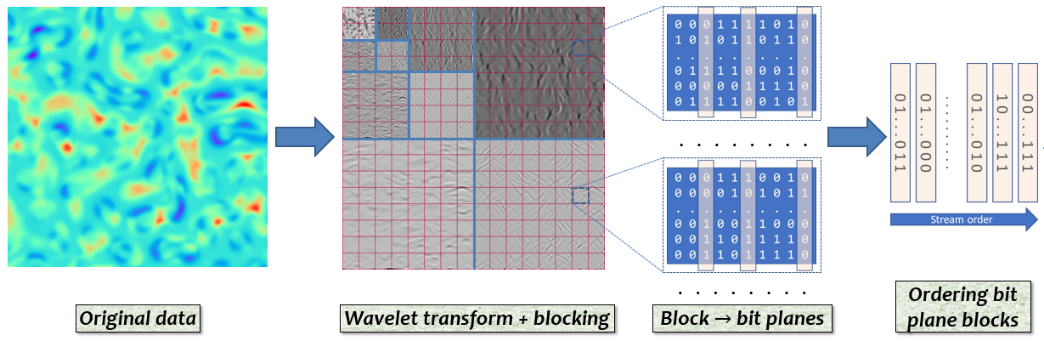
\includegraphics[width=\linewidth]{img/pipeline.png}
\caption{Our data streaming model (in 2D). The input is a regular grid of
floating-point samples; the output is a stream of packets. Different data
reduction schemes generate different streams.  The wavelet subbands are
separated by blue lines in the second image, with the coarsest subband at the
top left corner. Although not shown here, quantization and negabinary
convesion happen immediately after wavelet transform. \todo{TODO: revise this
figure}}\label{fig:pipeline}
\end{figure}

\subsection{Data-dependent and Data-independent Streams} \label{sec:static-dynamic-streams}

\newcommand {\mm}[1] {\ifmmode{#1}\else{\mbox{\(#1\)}}\fi}

\newcommand{\sopt}        {\mm{S_{\text{opt}}}\xspace}
\newcommand{\slvl}        {\mm{S_{\text{lvl}}}\xspace}
\newcommand{\sbit}        {\mm{S_{\text{bit}}}\xspace}
\newcommand{\swav}        {\mm{S_{\text{wav}}}\xspace}
\newcommand{\smag}        {\mm{S_{\text{mag}}}\xspace}
\newcommand{\wlvl}        {\mm{W_{\text{lvl}}}\xspace}
\newcommand{\wbit}        {\mm{W_{\text{bit}}}\xspace}
\newcommand{\wwav}        {\mm{W_{\text{wav}}}\xspace}
\newcommand{\wmag}        {\mm{W_{\text{mag}}}\xspace}
\newcommand{\err}         {\mm{\varepsilon}\xspace}

Although both the server and the client in our model can be on the same physical
machine, only the server has full knowledge of the data. Thus, when the client
receives a packet, it might not know where that packet should be deposited. A
common solution is to have both the client and the server agree beforehand on a
static ordering of packets, independent of the data. We use the term
\emph{data-independent streams} to refer to streams using this solution. In
contrast, for \emph{data-dependent streams}, \hbadd{additional mechanism is
needed to inform the client about the position of incoming packets.} \hbdel{the
client is assumed to ``magically'' know the positions of packets without
receiving this information from the server.}

A stream is an ordered collection of packets, $p_i$, sorted in descending order
of some associated weight, $W_i$. Thus, a stream can be characterized using a
weighting function.
%
We call the two sorting criteria, corresponding to two common data reduction
schemes in the literature, as \emph{by level} and \emph{by bit plane}.  The
\emph{by level} stream, \slvl, orders the packets strictly from coarser to
finer resolution levels. The weight function in this case is $\wlvl(p)=L-l(p)$,
where $l(p)$ is the subband index of $p$, and $L$ is the total number of
subbands. Within the same subband, without any assumption on the underlying
data, packets follow the row-major order of coefficients and then bit plane order
(from 0 to $B$) within each coefficient. The other common ordering, \emph{by
bit plane}, denoted as \sbit, proceeds strictly from higher ordered to
lower ordered bit planes. That is, $\wbit(p)=B-b(p)$, where $b(p)$ is the bit
plane index of $p$, and $B$ is the total number of bit planes. Within the same
bit plane, packets follow the subband order (from 0 to $L$), and then row-major
order in each subband. 
%
The streams \slvl and \sbit are designed to mimic the way data is accessed in
traditional methods that work either in resolution (\slvl) or in precision
(\sbit). 

We also define a third stream, which combines these two dimensions, and refer
to it as \emph{by wavelet norm}, \swav.  This stream orders packets using
weights $\wwav(p)=2^{B-1-b(p)}\times \norm{\omega_{l(p)}}^2$. The first term
captures the contribution of a bit on bit plane $b(p)$, and the second term
captures the contribution of a wavelet coefficient on subband $l(p)$, where
$\omega_{l(p)}$ refers to a wavelet basis function on subband $l(p)$. In the
wavelet representation, a function $f$ is written as a linear sum of wavelet
basis functions $\omega_i$: $f=\sum{c_i\omega_i}$, where $c_i$ are the
coefficients. Since basis functions in the same subband share the same norm,
$\wwav(p)$ is simply the contribution (in $L_2$ norm) of a bit on bit plane
$b_p$ and subband $l_p$, to the whole function $f$. To our knowledge, a data
reduction scheme based on \emph{by wavelet norm} was hinted at in
\todo{[CITE]}. \duong{if there is enough space, include here the formula to
compute the norm of basis functions, else put it in the appendix}

Another common data reduction technique, especially for transform-based data,
is one in which truncation happens leaving out coefficients of smallest
magnitudes. We model this scheme with a stream called \emph{by magnitude},
\smag. Here, the weight function is $\wmag(p)=\sum_{c\in
\text{block}(p)}\norm{c}^2$ (the sum is over all coefficients in the block that
contains packet $p$). If two packets have the same weight, they are ordered by
subband index, and then by bit plane. Unlike \slvl and \sbit, \smag
%\emph{by level} and \emph{by bit plane}, \emph{by magnitude} 
is data dependent, because the coefficient magnitudes are not known until after
the data has gone through the wavelet transform.

In general, data-dependent streams are better than data-independent streams in
theory, because they can prioritize important packets based on the actual data.
However, data-dependent streams are ill-suited for practical purposes, because
the cost of sending position information likely outweights any potential
benefit. Nevertheless, we study them for various reasons. First, the \emph{by
magnitude} scheme is well known in the literature. Second, data-dependent
streams can serve as a benchmark to evaluate the performance of their
data-independent counterparts. Finally, in addition to being data dependent,
streams can also be task dependent (\Cref{sec:data_dep_streams}), which may
provide insights on how data should be queried to perform certain analysis
tasks.

\subsection{Data-dependent, Task-optimized Streams} \label{sec:data_dep_streams}

Each analysis task potentially requires a fundamentally different stream for optimal results. Two
streams can be compared on the basis of how well they work for a given analysis task, provided that an
error metric for that task is well defined. This section aims to solve the problem of finding the
optimal (and data-dependent) stream, given a data set and such an error metric. Studying such a
stream is important because it serves not only as a benchmark, but also as a source of insights for
other, more practical streams for the same task.

Given the original data $f$ and its reconstructed approximation $f'$ using a subset of packets, 
let $q$ represent some quantity of interest (e.g., histogram, isocontour, etc.) computed on 
$f$ or $f'$. In
this paper, we use the terms ``quantity of interest'' and ``task'' interchangebly, with the
understanding that, e.g., if the task is extracting isocontours, then the quantity of interest is 
isocontours. For a given task $q$, we define an error metric $\err(q(f'),q(f))$ that is either common
or intuitive and simple while generalizable \hb{why do we need common, intuitive, or simple?}. Given a data set $f$, a task $q$, and an error metric $\err$, 
our goal is to generate a stream $\sopt$ that is optimal for $q$ with respect to $\err$.

\hbdel{
One way to define the ``optimal'' stream could be one that incurs the minimum error $\err$ at every
point. In trying to realize this definition, however, our experience has been that such a stream does not exist. 
Assume otherwise that the optimal stream exists; then by definition, it must be possible to
construct this stream (called $\sopt$) using the following greedy algorithm. Start with a pool
consisting of all packets, an all-zero function $f'$, and an empty $\sopt$. From the pool, pick
one packet $p$ that when applied to the current $f'$, would minimize $\err$. Remove $p$ from the pool,
add it to the end of $\sopt$, and update $f'$ using $p$. Repeat this process until the pool is
empty. This algorithm can encounter a situation in which the chosen packet $p$ contributes almost
nothing to $f'$, yet the error is minimized because it is kept approximately constant. In this case,
it is actually better to pick another packet that increases the error slightly, but otherwise
contributes more to $f'$. In optimization terms, it is necessary to follow a search direction
that increases the error slightly to avoid being stuck in a local minimum. This contradiction shows
that $s_{opt}$ does not exist, using the aforementioned definition of optimality.}
\hb{rephrased this paragraph as below}

\hbadd{One way to define the ``optimal'' stream could be one that incurs the minimum error $\err$ at every
intermediate $f'$. However, such a stream assumes the existence of a single global optimum, and may not 
exist. \todo{(don't think we need to describe the algorithm. just saying the greedy 
can get stuck in local minima should be sufficient.)}
Consider the following greedy algorithm for the construction of such a hypothetical stream.
Starting with an all-zero function $f'$, and an empty stream, append a new packet $p$ to the stream 
that when included in the current $f'$, would minimize $\err$. Repeat this process until the 
all data has been considered or the prescribed data budget has been fulfilled.
However, such a greedy approach could lead to a local minimum, and keep picking packets that contribute
almost nothing to $f'$.}

\hbadd{Instead, we consider \sopt} 
\hbdel{We can change the definition of $s_{opt}$}
to be a stream such that the area \hbadd{under the curve} \hbdel{bounded by its error
curve (when plotted) and the horizontal axis} \hbadd{of \err} is the smallest \hbadd{for all packets to be streamed}. 
However, this definition is of limited
usefulness in practice, because a stream should be able to terminate at any point, and it still
produces an error as small as possible. 
\hb{ok, this is now very confusing. why do we switch back and forth? why don't we discuss the area under the curve definition first?
leaving the rest of this subsection until we know what to do here} Therefore, instead of using this definition of optimality,
we slightly modify the greedy algorithm above to avoid local minima. We still start with a pool
consisting of all packets and an empty $s_{opt}$, but with a ``lossless'' $f'$ (i.e., $f'=f$), and
we build $s_{opt}$ back to front. In each step, the packet whose removal from $f'$ has the least
impact on the error $e$ is removed from both $f'$ and the pool, and inserted to the beginning of
$s_{opt}$. This algorithm solves the previous problem where unimportant packets were added to
$s_{opt}$ too early (i.e., the algorithm gets stuck in a local minimum). Here, packets chosen early
are actually unimportant, and will be put at the end of $s_{opt}$.

Unfortunately, we have found that this back-to-front greedy algorithm is too costly in practice.
Ignoring all the steps done in each iteration, this algorithm amounts to a 2-level nested loop
running for $n^2$ iterations, where $n$ is the total number of packets. With a $256^3$-size domain,
a packet size that spans $16^3$ coefficients, and $16$ bits of quantization, $n$ is 65536, so $n^2$
would be in the billions, which we have found to be prohibitively large. We have therefore adopted a
simplified version of this algorithm, where only one pass through the set of $n$ packets is needed.
The modified algorithm works as follows. In each iteration $i$, we disable (set to zero) a new
packet $p_i$ in $f'$, then compute and record the incurred error $e_i$. $p_i$ is enabled again in
$f'$ at the end of iteration $i$. After $n$ iterations, each packet has an associated weight $e_i$.
$s_{opt}$, then, is simply the sorted list of packets in decreasing order of the weights. This
simplified algorithm brings the running time from days down to minutes, while (by observation)
retaining the same quality for $s_{opt}$. The pseudocode of the algorithm is presented in~\Cref{alg:greedy}.

\begin{algorithm}[h]
  \small
  %\algsetup{linenosize=\small}
  \caption{Computing a task-optimized stream}
  \begin{algorithmic}[1]
    \Inputs{
			An original function $f$\\
			An unordered set of $n$ packets $P = \{p_i\}$, produced from $f$\\
			A quantity of interest $q$, and an error function $e$}
		\Initialize{A set of $n$ weights $\Gamma = \{\gamma_i\}$ }
		\For{each packet $p_i$}
			\State $p_i := 0$
      \State $P \rightarrow$ wavelet coefficients $W$ (inverse quantization and inverse negabinary transform)
			\State $W \rightarrow f'$ (inverse wavelet transform)
			\State $\gamma_i := e(q(f'),q(f))$			
			\State Restore $p_i$
		\EndFor
		\State Sort the $p_i$'s in descending order of $\gamma_i$.
		\Output{The $q$-optimized stream, which is the sorted $P$}
	\end{algorithmic}
	\label{alg:greedy}
\end{algorithm}

\subsection{Stream Signatures} \label{sec:stream-signature}

Denote the 2D space of bit planes versus subbands (or precision versus resolution) as $S_{L,B}$
(i.e., $S_{L,B}=\{(l,b) | 0\leq l\leq L, 0\leq b\leq B\}$). Unlike data-independent streams,
data-dependent streams do not impose a static ordering of packets in this space. Therefore, to
analyze this aspect of a data-dependent stream, we introduce the concept of a \emph{stream
signature}. Given a stream, a signature $A_{L,B}$ is an $L \times B$ matrix, whose $(l,b)$ element
is associated with $P_{l,b}$ --- the set of packets belonging to subband $l$ and bit plane $b$. In
particular, $A(l,b)$ is an integer in the $[0, B\times L)$ range that indicates, on average, the
position in which $P_{l,b}$ appear in the given stream. For example, the signature $A=\bigl[
\begin{smallmatrix}0 & 1 & 4\\ 2 & 3 & 5\end{smallmatrix}\bigr]$ indicates that the stream begins
with packets that lie on the first bit plane of the first subband, as $A(0,0)=0$. Those are followed
by packets on the second bit plane of the first subband ($A(0,1)=1$), and then the first bit plane of
the second subband ($A(1,0)=2$). Finally, the last group of packets comes from the third bit plane
of the second subband ($A(1,2)=5$). A stream's signature shows how the stream traverses the space
$S_{L,B}$. In this way, the signature concept can reveal the potentially different
resolution-versus-precision tradeoffs among $s_{opt}$ streams optimized for different tasks.

To compute a stream signature, we partition the whole domain (not individual subbands) into several
\emph{regions}, compute one signature per region, and average these local signatures. It is
only when packets are relatively well localized that their relative ordering in the $S_{L,B}$ space
becomes meaningful. For example, a packet at one corner of the domain can be streamed before one at
an opposite corner, but this fact contains no useful information. We define a region to be the
spatial volume that is covered by a packet in the coarsest subband. Algorithm~\ref{alg:signature}
lists the steps in detail.

\begin{algorithm}[h]
  \small
  \caption{Computing a stream signature}
  \begin{algorithmic}[1]
    \Inputs{
			A stream $P=\{p_i\}$\\}
		\Initialize{Per-region signature matrix $A_r:= 0$\\
		Global signature matrix $A := 0$}
		\For{each packet $p_i$ in $P$}
			\State Let $r$, $b$, $l$ be the region, bit plane, and subband that $p_i$ belongs
			\State $A_r(l,b) := A_r(l,b)+i$
		\EndFor
		\For{each region $r$}
			\State Sort the elements of $A_r$
			\State Assign each element of $A_r$ its index after sorting
			\State $A := A+A_r$
		\EndFor
		\State Sort the elements of $A$
		\State Assign each element of $A$ its index after sorting
		\Output{The signature matrix $A$}
	\end{algorithmic}
	\label{alg:signature}
\end{algorithm}

Finally, a signature can be used to construct a ``semi''-data-independent stream, denoted as
$s_{sig}$. This construction is done by iterating through each element $A(l,b)$ in ascending order, and adding
end of $s_{sig}$ all the packets in $P_{l,b}$. $s_{sig}$ is similar to purely data-independent
streams, in that the ordering of packets in the $S_{l,b}$ space is deterministic (governed by the
signature). However, this deterministic ordering must be established between the client and the
server through the transmission of the signature. This is not a hurdle in practice, because the size
of the signature should be negligible compared to the size of the data itself. In 3D, assuming 22
subbands and 32-bit quantized coefficients, a signature contains $1408 (=22\times 32\times 2)$
bytes. $s_{sig}$ has no element of spatial-adaptivity; hence it can serve as a bridge when comparing
the resolution-versus-precision tradeoffs between data-independent and data-dependent streams.
